\section{Influence of temperature on the response of a straight pipe}
\subsection{Meaning and significance of stress terms}
\subsubsection{Principal stress}
Principal stress is a measure which defines the maximum normal stress which may be applied to a body of interest and where that stress is located. %Principal stress acts on the principal plane (an oblique plane at some angle $\theta$) and has the condition that there is zero shear stress on this plane. The resultant normal stresses acting on the principal plane, $\sigma_n$, is the principal stress. The normal stress can take a maximum or minimum value.
In the 3D case, we find that there exist three principal planes (where the shear stress is zero), which are orthogonal and each have their own maximum / minimum normal stresses. From this, we can also find locations and magnitude for the maximum shear stress.

Consider the six components of the 3D solid stress tensor:
\begin{equation}
    \sigma_{ij} = \begin{bmatrix}
        \sigma_x  & \tau_{yx} & \tau_{zx} \\
        \tau_{xy} & \sigma_y  & \tau_{zy} \\
        \tau_{xz} & \tau_{yz} & \sigma_z
    \end{bmatrix}
\end{equation}
where the first subscript denotes the direction of the surface normal and the second the direction of the stress. For static equilibrium:
\begin{equation}
    \tau_{xy} = \tau_{yx} \qquad \tau_{xz} = \tau_{zx} \qquad \tau_{zy} = \tau_{yz}
\end{equation}
By rotating the coordinate axes of our 3D body, we can change the components of the solid stress tensor, whilst representing the same state of stress on the body. As our matrix is symmetric, we can calculate a set of orthogonal axes which result in all $\tau$ elements equalling zero. This set of axes is called the principal axes and by applying this transformation to our solid stress tensor, we find the eigenvalues of the matrix and the principal stresses. Hence:
\begin{gather}
    \boldsymbol{\sigma}_{ij} = \begin{bmatrix}
        \sigma_x  & \tau_{yx} & \tau_{zx} \\
        \tau_{xy} & \sigma_y  & \tau_{zy} \\
        \tau_{xz} & \tau_{yz} & \sigma_z
    \end{bmatrix} \xrightarrow{eigenvalues} \boldsymbol{\sigma}_{ij}' = \begin{bmatrix}
        \sigma_1 & 0        & 0        \\
        0        & \sigma_2 & 0        \\
        0        & 0        & \sigma_3
    \end{bmatrix}\\
    \det(\boldsymbol{\sigma} - \sigma \boldsymbol{I}) = 0
\end{gather}
where $\boldsymbol{I}$ is the identity matrix and $\sigma$ is the eigenvalue. The eigenvectors of the stress tensor, which correspond to the principal directions (the angles between the original (or base) coordinate axes and the new (or transformed) coordinate axes), can be found by solving the equation:
\begin{equation}
    (\boldsymbol{\sigma} - \sigma \boldsymbol{I})\boldsymbol{v} = \boldsymbol{0}
\end{equation}
where $\boldsymbol{v}$ is the eigenvector. This may also be written as:
\begin{align}
    \cos \alpha = \cos\left(n, \, x\right) & = l \\
    \cos \beta = \cos\left(n, \, y\right)  & = m \\
    \cos \gamma = \cos\left(n, \, z\right) & = n
\end{align}
where $n$ is the unit normal to the plane. We can now define the normal stress acting on any oblique plane:
\begin{equation}
    \sigma_{x'} = \sigma_xl^2 + \sigma_y m^2 +\sigma_zn^2 + 2\left(\tau_{xy}lm + \tau_{xy}mn + \tau_{xz}ln\right)
\end{equation}
We are interested in the maximum and / or minimum values of the normal stress acting on our body throughout the range of oblique planes. These maxima / minima are the principal stresses. This is determined by calculating the differentials of the above equations with respect to the direction cosines. We find that the principal stresses occur on planes where the shear stress is zero, as mentioned previously. The equations for in-plane principal stresses are shown below. The third stress is zero in plane stress conditions.
\begin{gather}
    \sigma_1 = \left(\frac{\sigma_x + \sigma_y}{2}\right)+ \sqrt{\left(\frac{\sigma_x - \sigma_y}{2} \right)^2+ \tau^2_{xy} }\\
    \sigma_2 = \left(\frac{\sigma_x + \sigma_y}{2}\right)- \sqrt{\left(\frac{\sigma_x - \sigma_y}{2} \right)^2+ \tau^2_{xy} }
\end{gather}

A key characterisation of the principal stress is that it acts in the normal direction to the principal plane - this is important to note as a distinction. The determination of the principal stresses (and maximum shear stress) is important for design purposes as it tells us whether a body would be able to withstand a design load at a given location.
\subsubsection{Von Mises stress}
Von Mises stress can be used to determine whether an isotropic and ductile material will yield under a complex loading condition. The von Mises stress equation is based on the principle that the failure of a material is dependent on the total amount of energy that is being absorbed by the material, rather than the individual stresses in each direction. The equation simplifies the complex stress state of a material, which is often composed of multiple stresses acting in different directions, into a single numerical value that is used to determine whether the material is likely to fail. A comparison between the material's yield stress and the von Mises stress allows the calculation of the von Mises Stress Criterion.

An equation for the von Mises stress is shown below.
\begin{equation}
    \sigma_{VM} = \sqrt{\frac{1}{2}\left[\left(\sigma_{x}-\sigma_y\right)^2 + \left(\sigma_y - \sigma_z\right)^2+\left(\sigma_z - \sigma_x\right)^2\right] + 3\left(\tau^2_{xy} + \tau^2_{yz}+\tau_{zx}^2\right)}
\end{equation}
However, we can also calculate the von Mises stress directly from the principal stresses (note that we may not do the reverse).
\begin{equation}
    \sigma_{VM} = \sqrt{\frac{1}{2}\left[\left(\sigma_1 - \sigma_2\right)^2 +\left(\sigma_2 - \sigma_3\right)^2 + \left(\sigma_3 - \sigma_1\right)^2 \right]}
\end{equation}

The von Mises stress is often used in engineering design to determine whether a material will fail under a given load. If the von Mises stress exceeds the yield strength of the material, plastic deformation is expected to occur. Therefore, designers can use the von Mises stress to ensure that their designs remain within the elastic limit of the material.
\subsubsection{Stress magnitude}
Stress magnitude refers to the amount or level of stress experienced by an object or system. Stress, in essence, describes the force per unit area acting on a material, and stress magnitude is determined by the magnitude of this force.
\subsection{Relationship between axial stress and temperature of length constrained 3D pipe}\label{part1b}
The derivation presented here concerns the thermal bowing of a laterally restrained beam or pipe subjected to a uniform temperature gradient. The derivation aims to obtain an equation that describes the lateral displacement of the beam due to the thermal load.

The starting point of the derivation is the expression for the displacement of a point in the beam. The displacement can be expressed as a function of the position along the beam, $x$, and two lateral coordinates, $y$ and $z$, as:
\begin{equation}
    u(x,y,z) = f(x) + yf_1(x) + zf_2(x)
\end{equation}
where $f(x)$ is the longitudinal displacement, $f_1(x)$ is the lateral slope, and $f_2(x)$ is the curvature.

The longitudinal strain in the beam can be expressed as the partial derivative of the displacement with respect to the longitudinal coordinate, $x$, as:
\begin{equation}
    \epsilon_{xx} = \frac{\partial u}{\partial x} = f'(x) + yf_1'(x) + zf_2'(x)
\end{equation}
The stress field in the beam can be expressed as a function of the longitudinal strain and the temperature distribution in the beam. Assuming that the temperature distribution is uniform and the longitudinal strain is solely due to thermal expansion, the stress field can be expressed as:
\begin{equation}
    \sigma_{xx} = E \left(\epsilon_{xx} - \alpha T\right)
\end{equation}
where $E$ is the modulus of elasticity of the material, $\alpha$ is the coefficient of thermal expansion, and $T$ is the temperature in the beam.

The equilibrium of forces and moments in the beam requires that the stress field integrates to zero over the cross-sectional area of the beam. Assuming that the temperature distribution is uniform, this condition can be expressed as:
\begin{align}
    \int \sigma_{xx} \dif A   & = 0 \\
    \int \sigma_{xx} y \dif A & = 0 \\
    \int \sigma_{xx} z \dif A & = 0
\end{align}
where $\dif A$ is an element of the cross-sectional area of the beam, and $y$ and $z$ are the lateral coordinates of the element.

The geometrical constraint is that the center of gravity of the cross-pipe must be located at the origin:
\begin{equation}
    \int y \dif A = \int z \dif A = 0
\end{equation}
Next, we consider the cross-pipe variation of temperature. The stress field in x-direction can be expressed as:
\begin{equation}
    \sigma_{xx} = -\alpha E\left(T - T_0\right) + \frac{I_yM_{Tz}-I_{yx}M_{Ty}}{I_yI_z-I^2_{yz}}y + \frac{I_yM_{Tz}-I_{yx}M_{Ty}}{I_yI_z-I^2_{yz}}z
\end{equation}
where $T$ is the temperature at any given point, and $T_0$ is the average temperature of the pipe. $I_z$, $I_y$ and $I_{yz}$ are the moments of inertia of the cross-sectional area with respect to yz, zx and xy planes respectively. $M_{Ty}$ and $M_{Tz}$ are the moments due to the variation of temperature.

For a pipe with a circular cross-section, $I_z$ and $I_y$ are equal, and $I_{yz}$ is zero. Hence, the stress field in the x-direction reduces to:
\begin{equation}
    \sigma_{xx} = -\alpha E \left(T - T_0\right) + \frac{M_{Tz}}{I_y}y
\end{equation}
We can now derive the equation for lateral displacement of the pipe. The lateral displacement is obtained by taking the second derivative of the displacement function with respect to $x$:
\begin{gather}
    \frac{\dif^2 v}{\dif x^2} = - \frac{M_{Tz}}{EI_z}\\
    \frac{\dif}{\dif x^2}\left(EI_z\frac{\dif^2 v}{\dif x^2}\right) + \frac{\dif^2 M_{Tz}}{\dif x^2} = F
\end{gather}
The tensile force $P$ and a tensile $P-\delta$ moment $Py$ over the length of the beam give us the equation governing the displacement of the beam:
\begin{equation}
    \frac{\dif^2 y}{\dif x^2} = \phi + \frac{Py}{EI}
\end{equation}
where $y(x)$ is the displacement of the beam at position $x$, $\phi$ is the lateral displacement due to the uniform thermal gradient, $E$ is the Young's modulus, $I$ is the second moment of area.

Using the expression for the moment, $M = EI \phi = EI\alpha T_{,y}$, where $\alpha$ is the coefficient of thermal expansion and $T_{,y}$ is the temperature gradient, we can obtain the value of $P$ as:
\begin{equation}
    P = \frac{EI\alpha T_{,y}}{y}
\end{equation}
Substituting this expression for $P$ into the equation for the displacement, we get:
\begin{equation}
    \frac{\dif^2 y}{\dif x^2} - k^2 y = \phi
\end{equation}
where $k = \sqrt{P/EI}$. The solution to this differential equation is given by:
\begin{equation}
    y(x) = -\frac{\phi}{k^2}\left(\frac{\cosh(kl) - 1}{\sinh(kl)}\sinh(kx)\cosh(kx)+1\right)
\end{equation}
where $l$ is the length of the beam. This equation gives the displacement of the beam at any point $x$ due to the uniform thermal gradient, and it shows that the maximum displacement occurs at the mid-span of the beam, where
\begin{equation}
    y(l/2) = \frac{\phi}{k^2 \tanh(kl/2)}
\end{equation}
Some approximations and limitations in this analysis come from the constrains used in this application. Usmani \textit{et al} outline that assuming that the axial restraints being perfectly rigid is practically impossible. Hence, an approach using axial restraints modelled with a spring with stiffness $k_s$ are more likely to be observed in real-world beams \cite{USMANI2001721}.
\subsection{3D pipe ANSYS}\label{part1c}
\subsubsection{Relationship between maximum stress in temperature range}
ANSYS was used to conduct analysis on a 3D pipe to determine the relationship between maximum stress $\sigma_m$ and $T-T_0$ over the temperature range specified as $T = \SI{-160}{\degree C}$ and $T = \SI{240}{\degree C}$ with $T_0 = \SI{22}{\degree C}$. The pipe external and internal diameters and length were specified as $D_e = \SI{813}{\milli\meter}$, $D_i = \SI{793.94}{\milli\meter}$ and $L = \SI{50}{\meter}$.

The geometry was constructed using ANSYS Discovery, and a test region of $\pm$ \SI{2.5}{\meter} from the centre of the pipe was chosen to probe the results. The setup is shown in Figure \ref{part1cSplitBody}
\begin{figure}[H]
    \centering
    \includegraphics[width=\textwidth]{img/part1c-3.png}
    \caption{Geometry of 3D pipe with probe region in the centre.}
    \label{part1cSplitBody}
\end{figure}
The constraints used in the analysis were carefully chosen to ensure that the resulting simulation was accurate. The use of `remote displacements' proved to provide the best representation of the support required for this analysis. These remote displacements were fixed in all axes and rotations. They were applied on the surfaces of both ends of the pipe. The remote point was chosen as the geometric centre of the pipe in the same plane (x-y). The support setup is shown in Figure \ref{supports}.
\begin{figure}[H]
    \centering
    \includegraphics[width = \textwidth]{img/part1c-4.png}
    \caption{Setup for remote displacement applied on the surface of both ends of 3D pipe.}
    \label{supports}
\end{figure}
Using fixed supports gave results with abnormal edge cases. ANSYS documentation has noted this issue with fixed supports applied on surfaces, edges and vertices. Fixed supports lead to singular stresses i.e. the stress approaches infinity near the fixed edge or vertex \cite{ansysDocumentation}. Another problem with fixed surfaces is the non-compliance in deformation in the x-y plane. We expect to see the pipe expand/contract in this plane due to thermal effects. Running the simulation with fixed supports showed that the main body of the pipe does expand and contract but the elements connected to the fixed surface at the ends of the pipe do not, leading to an abnormalities.

In comparison, remote displacements allowed the ends of the pipe to expand/contract in the x-y plane, but did not allow the pipe to move in the z-axis. This manifests in a variation in the stress at the ends of the pipe. This variation is relatively small, with variation of around 1\% from the average. As we are probing results from the centre of the pipe, this can be excluded from our discussion. A thermal condition was applied to the geometry spanning \SI{-160}{\degree C} to \SI{240}{\degree C}.

To determine the maximum stress $\sigma_m$, `Normal stress' was indexed in the solution. This was configured to determine the maximum normal stress in the z-axis. The simulation utilised 21 steps, resulting in linear temperature steps of \SI{20}{\degree C}. The results are shown in Figures \ref{part1cSimResults}, \ref{part1c2}, \ref{part1c3}.
\begin{figure}[H]
    \centering
    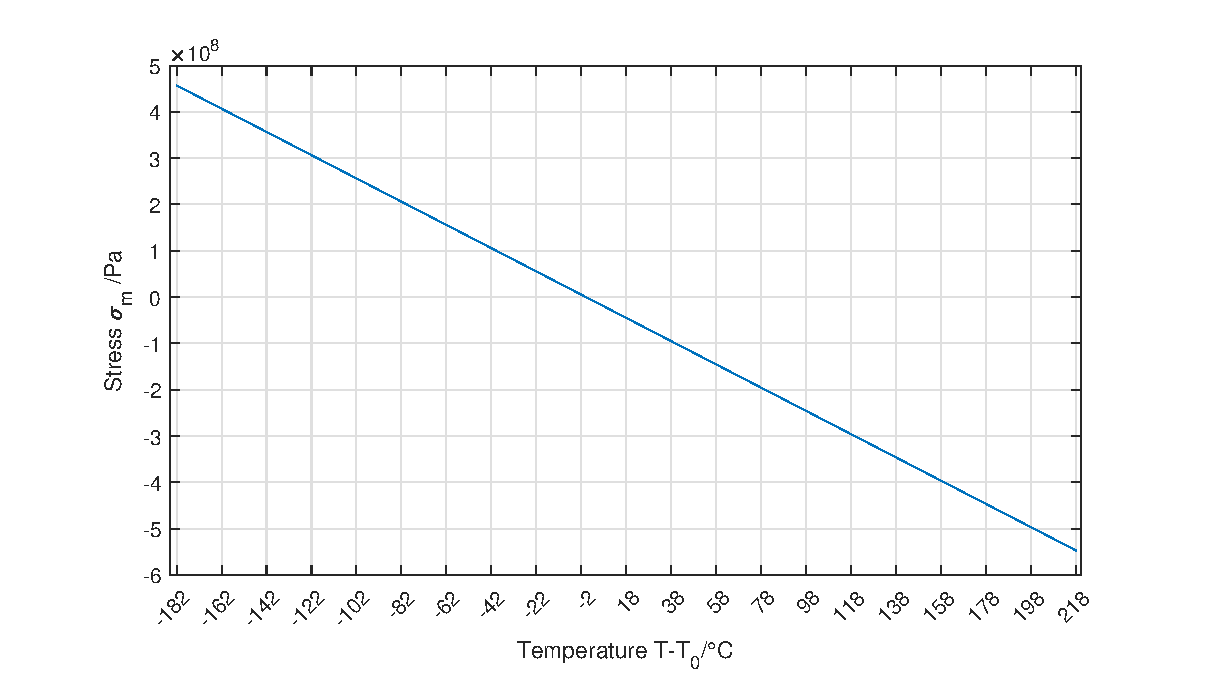
\includegraphics[width = 0.8\textwidth]{img/part1ci.eps}
    \caption{Plot of $\sigma_m$ in 3D pipe.}
    \label{part1cSimResults}
\end{figure}
\begin{figure}[H]
    \centering
    \includegraphics[width=\textwidth]{img/part1c-1.png}
    \caption{3D pipe at time-step 21, \SI{240}{\degree C}, axial stress.}
    \label{part1c2}
\end{figure}%
\begin{figure}[H]
    \centering
    \includegraphics[width=\textwidth]{img/part1c-2.png}
    \caption{3D pipe at time-step 21, \SI{240}{\degree C}, deformation. Note that the inside of the pipe has expanded less than the outside, i.e. the thickness of the pipe changes.}
    \label{part1c3}
\end{figure}%
\subsubsection{Comparison against theoretical result and discussion}
The theoretical result was calculated using (\ref{stressxx}). MATLAB was used to plot the results. Figure \ref{part1c4} shows the results from ANSYS and MATLAB plotted on the same graph. The variables used in the equation are shown in Table \ref{part1ciiVars}. The value of $M_{Tz}$ was set to zero in this case, as the bending moment is zero (from constraints).
\begin{equation}
    \sigma_{xx} = -\alpha E \left(T - T_0\right) + \frac{M_{Tz}}{I_y}y\label{stressxx}
\end{equation}
\begin{table}[H]
    \centering
    \begin{tabular}{@{}lll@{}}
        \toprule
        \textbf{Variable} & \textbf{Value}               & \textbf{Source}        \\
        \midrule
        $\alpha$          & \SI{1.2e-05}{\degree C^{-1}} & ANSYS Engineering Data \\
        $E$               & \SI{2e11}{\pascal}           & ANSYS Engineering Data \\
        $T_0$             & \SI{22}{\degree C}           & User-defined           \\
        \bottomrule
    \end{tabular}
    \caption{Values of variables used for theoretical calculation of 3D pipe stress.}
    \label{part1ciiVars}
\end{table}
\begin{figure}[H]
    \centering
    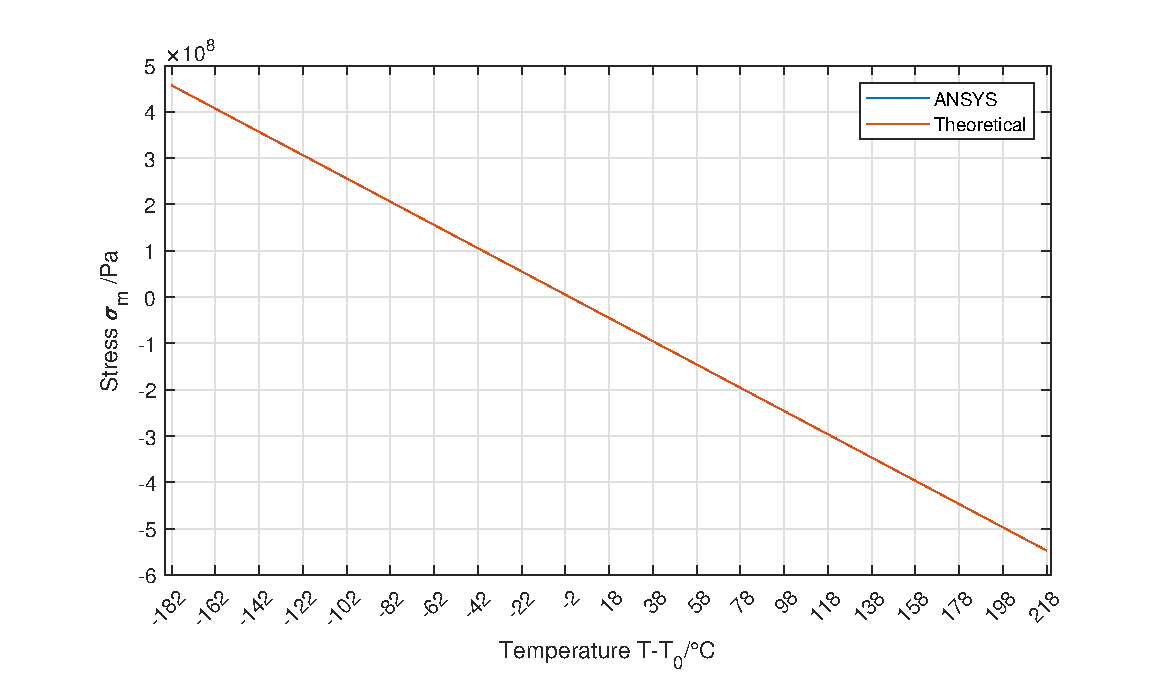
\includegraphics[width = \textwidth]{img/part1cii.eps}
    \caption{Plot of $\sigma_m$ in 3D pipe from ANSYS and theoretical calculation.}
    \label{part1c4}
\end{figure}
The results show a virtually identical stress magnitude. An average percentage of difference of \SI{6.12e-05}{\percent} was calculated for the results. The material properties were copied from ANSYS itself, and hence can be ruled out as a source of inaccuracy. The boundary conditions described above are the same between ANSYS and theoretical and can also be ruled out.

The slight difference in the numerical and theoretical results may arise from the numerical methods that ANSYS uses to solve the equations that describe the system. As noted previously, we see a very slight change in the thickness of the pipe, as the temperature varies and this could be contributing a small amount to the axial stress.
\subsection{1D pipe ANSYS}\label{part1d}
\subsubsection{Relationship between maximum stress in temperature range}
ANSYS was used to conduct analysis on a 1D pipe to determine the relationship between maximum stress $\sigma_m$ and $T-T_0$ over the temperature range specified as $T = \SI{-160}{\degree C}$ and $T = \SI{240}{\degree C}$ with $T_0 = \SI{22}{\degree C}$. The pipe external and internal diameters and length were specified as $D_e = \SI{813}{\milli\meter}$, $D_i = \SI{793.94}{\milli\meter}$ and $L = \SI{50}{\meter}$.

The geometry was constructed using ANSYS SpaceClaim, and a test region of $\pm$ \SI{2.5}{\meter} from the centre of the pipe was chosen to probe the results. The setup is shown in Figure \ref{part1dSplitBody}
\begin{figure}[H]
    \centering
    \includegraphics[width=\textwidth]{img/part1d-1.png}
    \caption{Geometry of 1D pipe with probe region in the centre. Mesh view was chosen for visualisation purposes.}
    \label{part1dSplitBody}
\end{figure}
`Fixed supports' were utilised at the ends of the pipe, to fix the displacement and rotation of the pipe in and around all axes. As the beam is modelled as a line segment with a given cross-section in 1D, there is no need to use a remote displacement to specify a particular constraint/behaviour in the x-y plane for the geometry. Two joint connections were also applied between each line segment to connect the geometry together. A thermal condition was applied to the geometry spanning \SI{-160}{\degree C} to \SI{240}{\degree C}. The setup is shown in Figure \ref{part1dSupports}.
\begin{figure}[H]
    \centering
    \includegraphics[width = \textwidth]{img/part1d-2.png}
    \caption{Setup for fixed supports applied on the ends of the pipe and thermal condition.}
    \label{part1dSupports}
\end{figure}
To determine the maximum stress $\sigma_m$, `Beam tool' was indexed in the solution. This was configured to determine the maximum normal stress in the z-axis using the `Direct stress' tool. The simulation utilised 21 steps, resulting in linear temperature steps of \SI{20}{\degree C}. The results are shown in Figures \ref{part1dSimResults}, \ref{part1d2}, \ref{part1d3}.
\begin{figure}[H]
    \centering
    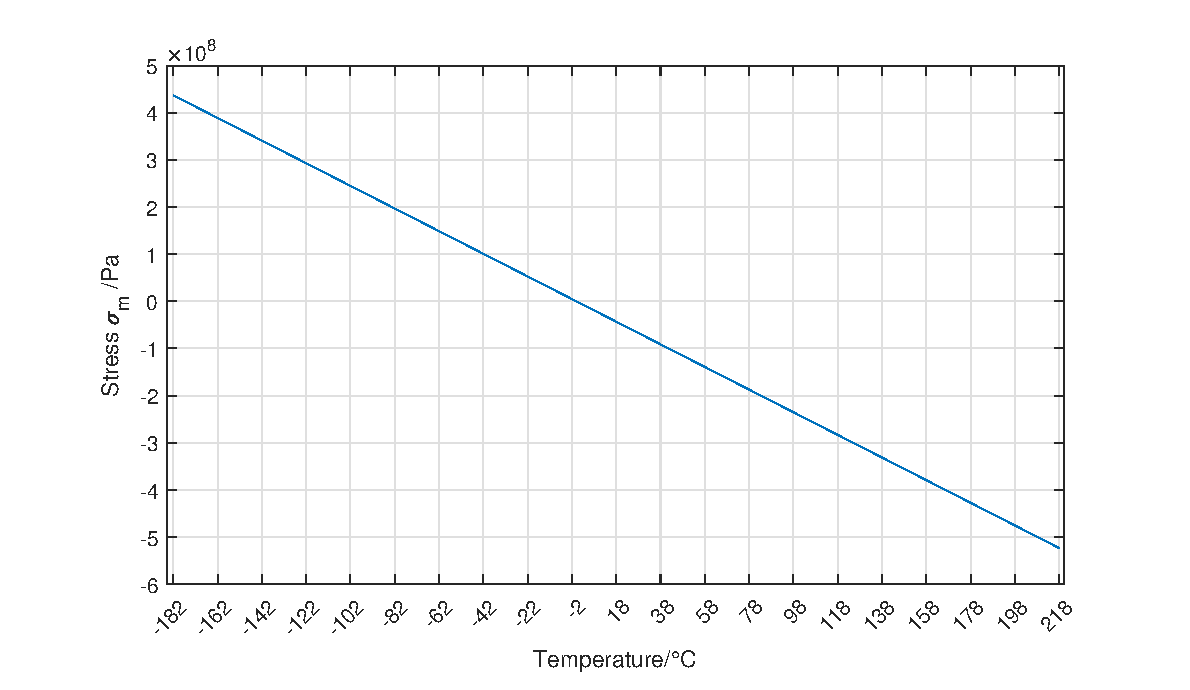
\includegraphics[width = \textwidth]{img/part1di.eps}
    \caption{Plot of $\sigma_m$ in 1D pipe.}
    \label{part1dSimResults}
\end{figure}
\begin{figure}[H]
    \centering
    \includegraphics[width=\textwidth]{img/part1d-4.png}
    \caption{1D pipe at time-step 21, \SI{240}{\degree C}, axial stress.}
    \label{part1d2}
\end{figure}%
\begin{figure}[H]
    \centering
    \includegraphics[width=\textwidth]{img/part1d-3.png}
    \caption{1D pipe at time-step 21, \SI{240}{\degree C}, deformation. Note that there is no deformation.}
    \label{part1d3}
\end{figure}%
\subsubsection{Comparison against theoretical result and discussion}
The theoretical result was calculated using (\ref{stressxx}). MATLAB was used to plot the results. Figure \ref{part1d4} shows the results from ANSYS and MATLAB plotted on the same graph. The variables used in the equation are the same as the ones used in the 3D analysis, shown in Table \ref{part1ciiVars}.
\begin{figure}[H]
    \centering
    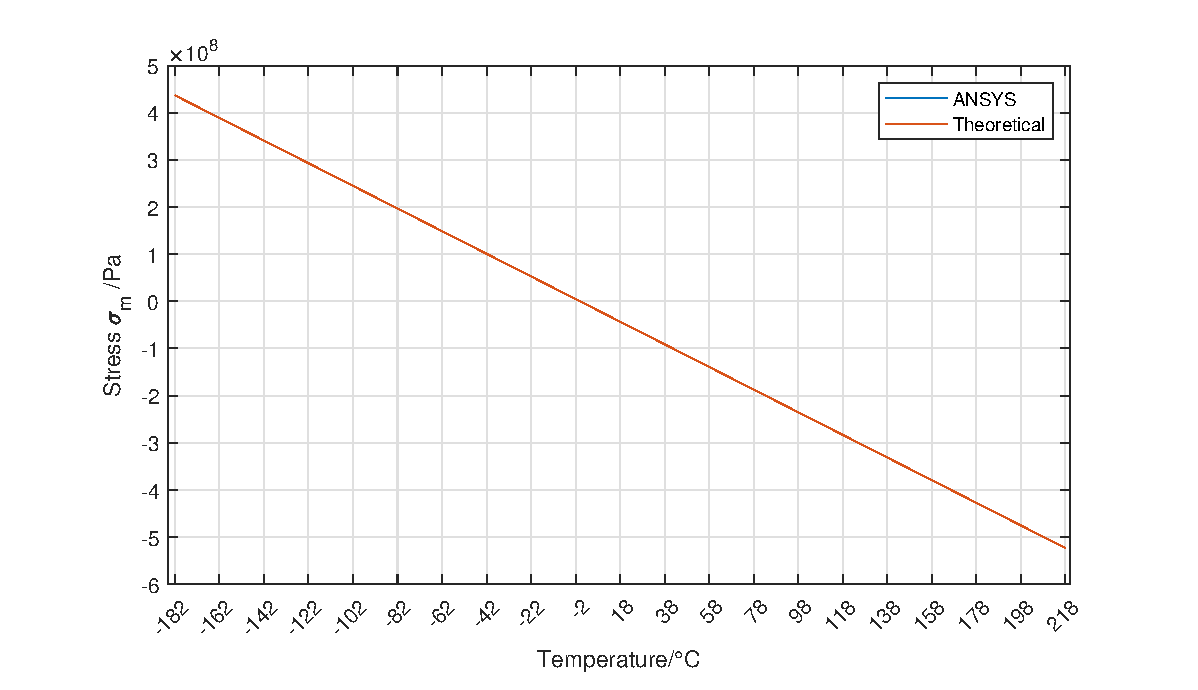
\includegraphics[width = \textwidth]{img/part1dii.eps}
    \caption{Plot of $\sigma_m$ in 1D pipe from ANSYS and theoretical calculation.}
    \label{part1d4}
\end{figure}
The results show an identical stress magnitude. An average percentage of difference of \SI{0}{\percent} was calculated for the results. As the simulation is utilising a 1D model, it is not accounting for changes in the thickness of the pipe (as this is absent from the simulation), hence, any contribution that may have on the axial stress is not captured in the simulation, giving us an exact result to the theoretical.
\subsection{Discussion}
\subsubsection{Difference and similarities between results from \ref{part1b}, \ref{part1c}, \ref{part1d} as pipe slenderness changes}
As the slenderness ratio changes ($L/D_e$), the accuracy of both simulations will change. The 1D model may become more accurate as the assumptions made for 1D modelling become more valid. Those assumptions are:
\begin{enumerate}
    \item The pipe is assumed to be perfectly straight and uniform in diameter
          \begin{itemize}
              \item This assumption is the same as the one used in our theoretical analysis. However, it must be noted that this would not be the case in any real-world scenario
          \end{itemize}
    \item The temperature and thermal expansion of the pipe (`thermal condition' in ANSYS) are assumed to be constant along the length of the pipe
          \begin{itemize}
              \item This assumption becomes more valid as the length of the pipe increases, since the temperature and thermal expansion are less likely to vary significantly along the length of the pipe in a real-world case
          \end{itemize}
    \item There are no axial, bending or torsional loads acting on the pipe
          \begin{itemize}
              \item As the slenderness increases, the effects of bending, torsion and transverse shear are (relatively) less significant, and the pipe can be better modelled as a 1D structure
          \end{itemize}
    \item The material properties of the pipe are assumed to be constant along its length
          \begin{itemize}
              \item This assumption is the same as that made in the theoretical. As previously noted, this would be impossible to achieve realistically
          \end{itemize}
    \item The pipe is assumed to be isotropic
\end{enumerate}
Another point of note is that the 1D simulation is highly dependent on a specific set of boundary and loading conditions. If the boundary/loading conditions were to be made more complex, our model may break down and lose accuracy, regardless of the pipe slenderness.

It may be expected that the 3D model become less accurate as the pipe slenderness changes. Due to the assumptions made in the theoretical analysis, the 3D model better captures the intricacies of the pipe's design, which may contribute to the result. Hence, we may see more deviation in our results as the pipe slenderness changes. The cause of those errors may be:
\begin{enumerate}
    \item Boundary conditions: the accuracy of the simulation is highly dependent on the accuracy and validity of the boundary conditions applied to the model. As noted previously, the differences between using fixed supports and remote displacement boundary conditions can change our results to a notable degree. As the pipe slenderness changes, it may be increasingly difficult to apply realistic (and hence valid) boundary conditions, leading to inaccuracies
    \item Numerical errors: As the pipe slenderness increases, the number of elements required to accurately model the geometry also increases. This can result in numerical errors arising from insufficient element density, if a proper mesh convergence test is not performed
    \item Assumptions: while the 3D simulation allows for more complex modelling than the 1D simulation, there are still assumptions made in the modelling process. E.g. the 3D simulation assumes perfect straightness, isotropy, and uniformity in diameter, which is unrealistic. As the pipe becomes longer, small imperfections may become more significant and affect the accuracy of the simulation
\end{enumerate}
In conclusion, the accuracy of simulations of a pipe subjected to temperature changes varies depending on the slenderness ratio ($L/D_e$) and the modelling approach used. The theoretical analysis provides a simplified representation of the problem and makes several assumptions. As the slenderness ratio increases, the 1D modelling approach becomes more valid, since the assumptions made become more accurate. However, this approach still makes some simplifications and may not account for certain effects. The 3D modelling approach provides a more accurate representation of the problem, but as the slenderness ratio increases, the accuracy decreases due to the increasing complexity and the limitations of the modelling software. Therefore, the choice of modelling approach should be based on the specific problem and the required level of accuracy.
\subsubsection{Model errors encountered using ANSYS Static Structural model}
When using ANSYS static structural to model a pipe under various slenderness ratios, there are several model errors that may occur, resulting in reduced accuracy of the simulation.

As the slenderness of the pipe increases, the accuracy of the 3D model decreases due to the assumption of a constant cross-section. In reality, as the pipe becomes more slender, there may be non-uniform changes in diameter, wall thickness, and even curvature, which the 3D model cannot account for. This leads to errors in the simulation results, such as incorrect stress distributions and deformations.

Increasing the slenderness ratio can lead to a number of errors related to the finite element method (FEM) calculations performed by the software. For example, the number of elements required to discretise the pipe may become too large, resulting in computational inefficiency and increased runtime. This can also lead to the model becoming numerically unstable, as the stiffness matrix may become ill-conditioned due to the high aspect ratio of the elements. Additionally, there may be difficulties in accurately capturing the effects of bending, torsion, and transverse shear forces on the pipe, leading to errors in the stress and strain fields. These errors can be exacerbated by the assumptions made in the 1D modelling approach, such as the assumption of uniform temperature and thermal expansion along the length of the pipe.
Finally, the ANSYS static structural model also assumes that there are no axial, bending, or torsional loads acting on the pipe. In reality, the pipe may be subjected to some degree of loading, which can lead to errors in the simulation results.